
% This LaTeX was auto-generated from MATLAB code.
% To make changes, update the MATLAB code and republish this document.

\documentclass{article}
\usepackage{graphicx}
\usepackage{color}

\sloppy
\definecolor{lightgray}{gray}{0.5}
\setlength{\parindent}{0pt}

\begin{document}

    
    

\section*{3. Chebyshev polynomials and series}

\begin{verbatim}
ATAPformats
\end{verbatim}
\begin{par}

Throughout applied mathematics, one encounters three closely analogous
canonical settings associated with the names of Fourier, Laurent, and
Chebyshev.  In fact, if we impose certain symmetries in the Fourier and
Laurent cases, the analogies become equivalences.
The Chebyshev setting is the one of central interest in this book,
concerning a variable $x$ and a function $f$ defined on $[-1,1]$:
$$ \hbox{\em Chebyshev:}\quad x\in [-1,1], \quad f(x)\approx \sum_{k=0}^n
a_kT_k(x). \eqno (3.1) $$
Here $T_k$ is the $k$th Chebyshev polynomial, which we shall discuss in
a moment.
For the equivalent Laurent problem, let $z$ be a
variable that ranges over the unit circle in the complex plane.
Given $f(x)$, define a transplanted function $F(z)$ on the
unit circle by the condition $F(z)=f(x)$, where
$x = (z+z^{-1})/2$ as in (2.1).  Note that this means that there are
two values of $z$ for each value of $x$, and $F$ satisfies the
symmetry property $F(z) = F(z^{-1})$.  The series now involves a
polynomial in both $z$ and $z^{-1}$, known as a {\em Laurent polynomial:}
$$ \hbox{\em Laurent:}\quad |z|=1, \quad F(z) = F(z^{-1}) \approx
{1\over 2} \sum_{k=0}^n
a_k(z^k + z^{-k}).  \eqno (3.2) $$
For the equivalent Fourier problem, let $\theta$ be a variable
that ranges over $[-\pi,\pi]$, which we regard as a $2\pi$-periodic domain.
Transplant $f$ and $F$ to a function ${\cal F}$ defined
on $[-\pi,\pi]$ by setting ${\cal F}(\theta) = F(e^{i\theta}) =
f(\cos(\theta))$ as in (2.2).  Now we have a 1-to-1 correspondence
$z = e^{i\theta}$ between $\theta$ and $z$ and a 2-to-1
correspondence between $\theta$ and $x$, with the symmetry
${\cal F}(\theta) = {\cal F}(-\theta)$, and the series is a
trigonometric polynomial:
$$ \hbox{\em Fourier:} \quad \theta\in[-\pi,\pi], \quad{\cal F}(\theta) =
{\cal F}(-\theta) \approx {1\over 2} \sum_{k=0}^n
a_k(e^{ik\theta} + e^{-ik\theta}). \eqno (3.3) $$
One can carry (3.1)--(3.3) further by introducing canonical systems
of grid points in the three settings.  We have already seen
the $(n+1)$-point Chebyshev grid,
$$ \hbox{\em Chebyshev points:}\quad x_j = \cos(\kern .5pt j\pi/n), \quad 0\le j \le n,
\eqno (3.4) $$
and we have interpreted these in terms of the $(2n)$th roots of
unity:
$$ \hbox{\em Roots of unity:}\quad z_j = e^{ij\pi/n}, \quad -n+1\le j \le n.
\eqno (3.5) $$
These grids are transplants of the set of
$2n$ equispaced points in $[-\pi,\pi]$:
$$ \hbox{\em Equispaced points:}\quad \theta_j = j\pi/n, \quad -n+1\le j \le n.
\eqno (3.6) $$

\end{par} \vspace{1em}
\begin{par}
All three of these settings are unassailably important. Real analysts cannot do without Fourier, complex analysts cannot do without Laurent, and numerical analysts cannot do without Chebyshev. Moreover, the mathematics of the connections between the three frameworks is beautiful. But all this symmetry presents an expository problem.  Without a doubt, a fully logical treatment should consider $x$, $z$ and $\theta$ in parallel. Each theorem should appear in three forms.  Each application should be one of a trio.
\end{par} \vspace{1em}
\begin{par}
It was on this basis that I started to write a book in 2008. The symmetries were elegant, but as the chapters accumulated, I came to realize that this would be a very long book and not a lovable one.  The excellent logic was just a dead weight.  The next year, I started again with the decision that the book would focus on $x\in [-1,1]$. This is the setting closest to much of approximation theory and numerical analysis, and it has a further special feature: it is the one least familiar to people.  Nobody is surprised if you compute a Fourier transform of a million points, but the fact that you can compute a polynomial interpolant through a million Chebyshev points surprises people indeed.
\end{par} \vspace{1em}
\begin{par}
Here then is the mathematical plan for this book.  Our central interest will be the approximation of functions $f(x)$ on $[-1,1]$.  When it comes to deriving formulas and proving theorems, however, we shall generally transplant to $F(z)$ on the unit circle so as to make the tools of complex analysis most conveniently available.
\end{par} \vspace{1em}
\begin{par}
Now let us turn to the definitions, already implicit in (3.1)--(3.3). The $k\kern -3pt$ th \textit{Chebyshev polynomial} can be defined as the real part of the function $z^k$ on the unit circle:
\end{par} \vspace{1em}
\begin{par}
 \vskip -1em
$$ x = \hbox{Re}(z) = {\textstyle{1\over 2}} (z+z^{-1})
= \cos \theta, \quad \theta = \cos^{-1}x, \eqno (3.7) $$
\vspace{-0.5em}
$$ T_k(x) = \hbox{Re}(z^k) = {\textstyle{1\over 2}}(z^k + z^{-k})
= \cos(k\theta).  \eqno (3.8) $$
\vspace{-1.5em} 
\end{par} \vspace{1em}
\begin{par}
(Chebyshev polynomials were introduced by Chebyshev in the 1850s, though without the connection to the variables $z$ and $\theta$ [Chebyshev 1854 \& 1859].  The label $T$ was apparently chosen by Bernstein, following French transliterations such as ``Tchebischeff.'')  The Chebyshev polynomials are a family of orthogonal polynomials with respect to a certain weight function (Exercise 3.7), but we shall not make much use of orthogonality until Chapters 17--19.
\end{par} \vspace{1em}
\begin{par}

It follows from (3.8) that $T_k$ satisfies $-1\le T_k(x) \le 1$ for
$x\in[-1,1]$ and takes alternating values $\pm 1$ at the $k+1$ Chebyshev
points. What is not obvious is that $T_k$ is a polynomial. We
can verify this property by the computation
$$ {\textstyle{1\over 2}}(z+z^{-1})(z^k + z^{-k})
= {\textstyle{1\over 2}}(z^{k+1}+z^{-k-1})
+ {\textstyle{1\over 2}}(z^{k-1}+z^{-k+1}) $$
for any $k\ge 1$, that is,
$$ 2xT_k(x) = T_{k+1}(x) + T_{k-1}(x), \eqno (3.9) $$
or in other words
$$ T_{k+1}(x) = 2xT_k(x) - T_{k-1}(x). \eqno (3.10) $$
\vspace{-1.5em} 
\end{par} \vspace{1em}
\begin{par}
By induction, this three-term recurrence relation implies that for each $k\ge 1$, $T_k$ is a polynomial of degree exactly $k$ with leading coefficient $2^{k-1}$. In Chapters 18 and 19 the coefficients of this recurrence will be taken as the entries of a ``colleague matrix,'' whose eigenvalues can be computed to find roots of polynomials or quadrature nodes.
\end{par} \vspace{1em}
\begin{par}

The Chebfun command \verb|chebpoly(n)| returns the chebfun corresponding
to $T_n$.\footnote{The name of the software system is Chebfun, with a
capital C.  A representation of a particular function in Chebfun is
called a chebfun, with a lower-case c.} Here for example are
$T_1,\dots,T_6$:

\end{par} \vspace{1em}
\begin{par}
 \vskip -2em 
\end{par} \vspace{1em}
\begin{verbatim}
FS = 'fontsize';
for n = 1:6
    T{n} = chebpoly(n);
    subplot(3,2,n), plot(T{n}), axis([-1 1 -1 1])
    text(.7,.41,'T',FS,10), text(.78,.24,int2str(n),FS,7)
end
\end{verbatim}

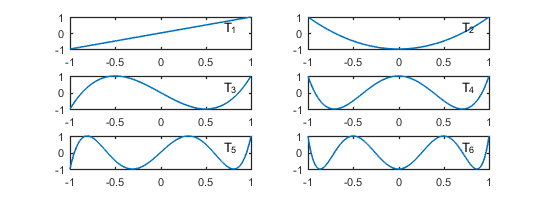
\includegraphics [width=4in]{chap3_01.png}
\begin{par}
 \vskip 1pt 
\end{par} \vspace{1em}
\begin{par}
These plots do not show the Chebyshev points, which are the extremes of each curve: thus the numbers of Chebyshev points in the six plots are 2, 3, 4, 5, 6, and 7.
\end{par} \vspace{1em}
\begin{par}

Here are the coefficients of these polynomials with respect to the
monomial basis $1,x,x^2,\dots.$\ \ As usual, Matlab orders coefficients
from highest degree down to degree zero.

\end{par} \vspace{1em}
\begin{par}
 \vskip -2em 
\end{par} \vspace{1em}
\begin{verbatim}
for n = 1:6, disp(poly(T{n})), end
\end{verbatim}

        \color{lightgray} \begin{verbatim}     1     0
     2     0    -1
     4     0    -3     0
     8     0    -8     0     1
    16     0   -20     0     5     0
    32     0   -48     0    18     0    -1
\end{verbatim} \color{black}
    \begin{par}
So, for example, $$ T_5(x) = 16x^5 - 20 x^3 + 5x. $$ The monomial basis is familiar and comfortable, but you should never use it for numerical work with functions on an interval.  Use the Chebyshev basis instead (Exercise 3.8). (If the domain is $[a,b]$ rather than $[-1,1]$, the Chebyshev polynomials must be scaled accordingly, and Chebfun does this automatically when it works on other intervals.)  For example, $x^5$ has the Chebyshev expansion $$ x^5 = {5\over 80}T_5(x) +  {5\over 16} T_3(x) + {5\over 8} T_1(x). $$ We can calculate such expansion coefficients by using the command \texttt{chebpoly(p)}, where $p$ is the chebfun whose coefficients we want to know:
\end{par} \vspace{1em}
\begin{par}
 \vskip -2em 
\end{par} \vspace{1em}
\begin{verbatim}
format short, x = chebfun('x'); chebpoly(x.^5)
\end{verbatim}

        \color{lightgray} \begin{verbatim}ans =
    0.0625         0    0.3125         0    0.6250         0
\end{verbatim} \color{black}
    \begin{par}
Any polynomial $p$ can be written uniquely like this as a finite Chebyshev series: the functions $T_0(x), T_1(x), \dots , T_n(x)$ form a basis for ${\cal P}_n$. Since $p$ is determined by its values at Chebyshev points, it follows that there is a one-to-one linear mapping between values at Chebyshev points and Chebyshev expansion coefficients. This mapping can be applied in $O(n\log n)$ operations with the aid of the Fast Fourier Transform (FFT) or the Fast Cosine Transform, a crucial observation for practical work that was perhaps first made by Ahmed and Fisher and Orzsag around 1970 [Ahmed \& Fisher 1970, Orszag 1971a and 1971b, Gentleman 1972b, Geddes 1978].  This is what Chebfun does every time it constructs a chebfun.  We shall not give details.
\end{par} \vspace{1em}
\begin{par}
Just as a polynomial $p$ has a finite Chebyshev series, a more general function $f$ has an infinite Chebyshev series.  Exactly what kind of ``more general function'' can we allow? For an example like $f(x) = e^x$ with a rapidly converging Taylor series, everything will surely be straightforward, but what if $f$ is merely differentiable rather than analytic?  Or what if it is continuous but not differentiable? Analysts have studied such cases carefully, identifying exactly what degrees of smoothness correspond to what kinds of convergence of Chebyshev series. We shall not concern ourselves with trying to state the sharpest possible result but will just make a particular assumption that covers most applications. We shall assume that $f$ is \textit{Lipschitz continuous} on $[-1,1]$. Recall that this means that there is a constant $C$ such that $|f(x) - f(y)| \le C |x-y|$ for all $x,y \in [-1,1]$. Recall also that a series is \textit{absolutely convergent} if it remains convergent if each term is replaced by its absolute value, and that this implies that one can reorder the terms arbitrarily without changing the result. Such matters are discussed in analysis textbooks such as [Rudin 1976].
\end{par} \vspace{1em}
\begin{par}
Here is our basic theorem about Chebyshev series and their coefficients.
\end{par} \vspace{1em}
\begin{par}
\textbf{Theorem 3.1. Chebyshev series.} \textit{If $f$ is Lipschitz continuous on $[-1,1]$, it has a unique representation as a Chebyshev series,}
\end{par} \vspace{1em}
\begin{par}
 \em \vspace{-1.5em}
$$ f(x) = \sum_{k=0}^\infty  a_k T_k(x), \eqno (3.11) $$
which is absolutely and uniformly convergent,
and the coefficients are given for $k\ge 1$ by the formula
$$ a_k = {2\over\pi} \int_{-1}^1 {f(x) T_k(x)\over \sqrt{1-x^2}} dx,
\eqno (3.12) $$
and for $k=0$ by the same formula with the factor $2/\pi$ changed to $1/\pi$.
\vspace{-.5em} 
\end{par} \vspace{1em}
\begin{par}
\textit{Proof.} Formula (3.12) will come from the Cauchy integral formula, and to make this happen, we begin by transplanting $f$ to $F$ on the unit circle as described above: $F(z) = F(z^{-1}) = f(x)$ with $x = \hbox{Re}\,z = (z+z^{-1})/2$. To convert between integrals in $x$ and $z$, we have to convert between $dx$ and $dz$: $$ dx = \textstyle{1\over 2} (1-z^{-2}) \, dz = \textstyle{1\over 2} z^{-1}(z-z^{-1}) \, dz. $$ Since $$ {\textstyle{1\over 2}} (z-z^{-1}) = i\kern .7pt\hbox{Im}\, z = \pm i \sqrt{1-x^2}, $$ this implies $$ dx = \pm i\kern .7pt z^{-1}\sqrt{1-x^2} \, dz. $$ In these equations the plus sign applies for $\hbox{Im}\, z\ge 0$ and the minus sign for $\hbox{Im}\, z\le 0$.
\end{par} \vspace{1em}
\begin{par}
These formulas have implications for smoothness. Since $\sqrt{1-x^2} \le 1$ for all $x \in [-1,1]$, they imply that if $f(x)$ is Lipschitz continuous, then so is $F(z)$. By a standard result in Fourier analysis, this implies that $F$ has a unique representation as an absolutely and uniformly convergent Laurent series on the unit circle, $$ F(z) = {1\over 2} \sum_{k=0}^\infty a_k (z^k + z^{-k}) = \sum_{k=0}^\infty a_k T_k(x). $$ Recall that a \textit{Laurent series} is an infinite series in both positive and negative powers of $z$, and that if $F$ is analytic, such a series converges in the interior of an annulus. A good treatment of Laurent series for analytic functions can be found in [Markushevich 1985]; see also other complex variables texts such as [Hille 1973, Priestley 2003, Saff \& Snider 2003].
\end{par} \vspace{1em}
\begin{par}

The $k$th Laurent coefficient of a Lipschitz continuous function $G(z) =
\sum_{k=-\infty}^\infty b_k z^k$ on the unit circle can be computed by
the Cauchy integral formula,
$$ b_k={1\over 2\pi i}\int_{|z|=1}z^{-1-k}G(z)\,dz. $$
(We shall make more substantial use of the Cauchy integral formula in
Chapters 11--12.) The notation $|z|=1$ indicates that the contour
consists of the unit circle traversed once in the positive
(counterclockwise) direction. Here we have a function $F$ with the
special symmetry property $F(z) = F(z^{-1})$, and we have also introduced
a factor $1/2$ in front of the series.  Accordingly, we
can compute the coefficients $a_k$ from either of two contour integrals,
$$ a_k={1\over\pi i}\int_{|z|=1}z^{-1+k}F(z)\,dz
={1\over\pi i}\int_{|z|=1}z^{-1-k}F(z)\,dz, \eqno (3.13) $$
with $\pi i$ replaced by $2\pi i$ for $k=0$.

\end{par} \vspace{1em}
\begin{par}

In particular, we can get a formula for $a_k$ that is symmetric
in $k$ and $-k$ by combining the two integrals like this:
$$ a_k={1\over 2\pi i}\int_{|z|=1}(z^{-1+k}+z^{-1-k})F(z)\,dz = {1\over \pi i}
\int_{|z|=1} z^{-1}\,T_k(x) F(z) \,dz, \eqno (3.14) $$
with $\pi i$ replaced by $2\pi i$ for $k=0$. Replacing $F(z)$ by $f(x)$
and $z^{-1} dz$ by $-i\,dx/(\pm \sqrt{1-x^2})$ gives
$$ a_k = -{1\over \pi} \int_{|z|=1}
{f(x) T_k(x)\over \pm \sqrt{1-x^2}} \,dx, $$ with $\pi$ replaced by
$2\pi$ for $k=0$.  We have now almost entirely converted to the $x$
variable, except that the contour of integration is still the circle
$|z|=1$.  When $z$ traverses the circle all the way around in the
positive direction, $x$ decreases from $1$ to $-1$ and then increases
back to $1$ again. At the turning point $z=x=-1$, the $\pm$ sign attached
to the square root switches from $+$ to $-$.  Thus instead of cancelling,
the two traverses of $x\in[-1,1]$ contribute equal halves to $a_k$.
Converting to a single integration from $-1$ to $1$ in the $x$ variable
multiplies the integral by $-1/2$, hence multiplies the formula for $a_k$
by $-2$, giving (3.12).
$~\hbox{\vrule width 2.5pt depth 2.5 pt height 3.5 pt}$

\end{par} \vspace{1em}
\begin{par}
We now know that any function $f$, so long as it is Lipschitz continous, has a Chebyshev series. Chebfun represents a function as a finite series of some degree $n$, storing both its values at Chebyshev points and also, equivalently, their Chebyshev coefficients.  How does it figure out the right value of $n$?  Given a set of $n+1$ samples, it converts the data to a Chebyshev expansion of degree $n$ and examines the resulting Chebyshev coefficients.  If several of these in a row fall below a relative level of approximately $10^{-15}$, then the grid is judged to be fine enough. For example, here are the Chebyshev coefficients of the chebfun corresponding to $e^x$:
\end{par} \vspace{1em}
\begin{par}
 \vskip -2em 
\end{par} \vspace{1em}
\begin{verbatim}
f = exp(x); a = chebpoly(f); format long, a(end:-1:1)'
\end{verbatim}

        \color{lightgray} \begin{verbatim}ans =
   1.266065877752008
   1.130318207984970
   0.271495339534077
   0.044336849848664
   0.005474240442094
   0.000542926311914
   0.000044977322954
   0.000003198436462
   0.000000199212481
   0.000000011036772
   0.000000000550590
   0.000000000024980
   0.000000000001039
   0.000000000000040
   0.000000000000001
\end{verbatim} \color{black}
    \begin{par}
Notice that the last coefficient is about at the level of machine precision.
\end{par} \vspace{1em}
\begin{par}
For complicated functions it is often more interesting to plot the coefficients than to list them.  For example, here is a function with a number of wiggles:
\end{par} \vspace{1em}
\begin{par}
 \vskip -2em 
\end{par} \vspace{1em}
\begin{verbatim}
f = sin(6*x) + sin(60*exp(x));
clf, plot(f), title('A function with wiggles',FS,9)
\end{verbatim}

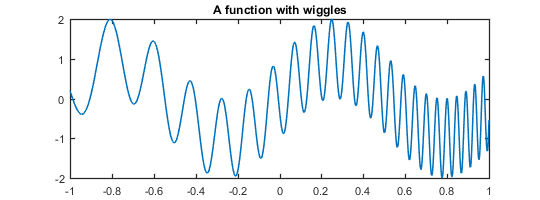
\includegraphics [width=4in]{chap3_02.png}
\begin{par}
 \vskip 1pt 
\end{par} \vspace{1em}
\begin{par}
If we plot the absolute values of the Chebyshev coefficients, here is what we find:
\end{par} \vspace{1em}
\begin{par}
 \vskip -2em 
\end{par} \vspace{1em}
\begin{verbatim}
a = chebpoly(f); semilogy(abs(a(end:-1:1)),'m')
grid on, title('Absolute values of Chebyshev coefficients',FS,9)
\end{verbatim}

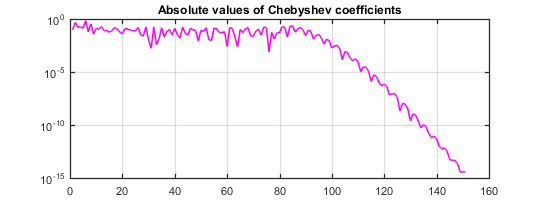
\includegraphics [width=4in]{chap3_03.png}
\begin{par}
 \vskip 1pt 
\end{par} \vspace{1em}
\begin{par}
One can explain this plot as follows.  Up to degree about $k=80$, a Chebyshev series cannot resolve $f$ much at all, for the oscillations occur on too short wavelengths.  After that, the series begins to converge rapidly.  By the time we reach $k=150$, the accuracy is about 15 digits, and the computed Chebyshev series is truncated there. We can find out exactly where the truncation took place with the command \texttt{length(f)}:
\end{par} \vspace{1em}
\begin{par}
 \vskip -2em 
\end{par} \vspace{1em}
\begin{verbatim}
length(f)
\end{verbatim}

        \color{lightgray} \begin{verbatim}ans =
   151
\end{verbatim} \color{black}
    \begin{par}
This tells us that the chebfun is a polynomial interpolant through 151 points, that is, of degree 150.
\end{par} \vspace{1em}
\begin{par}
 Without giving all the engineering details, here is a fuller
description of how Chebfun constructs its approximation. First it
calculates the polynomial interpolant through the function sampled at 9
Chebyshev points, i.e., a polynomial of degree 8, and checks whether the
Chebyshev coefficients appear to be small enough.  For the example just
given, the answer is no.  Then it tries 17 points, then 33, then 65, and
so on.  In this case Chebfun judges at 257 points that the Chebyshev
coefficients have fallen to the level of rounding error. At this
point it truncates the tail of terms deemed to be negligible, leaving a
series of 151 terms (Exercise 3.13). The corresponding degree 150
polynomial is then evaluated at 151 Chebyshev points via FFT, and these
151 numbers become the data defining this particular chebfun. Engineers
would say that the signal has been {\em downsampled\/} from 257 points to
151. 
\end{par} \vspace{1em}
\begin{par}
For another example we consider a function with two spikes:
\end{par} \vspace{1em}
\begin{par}
 \vspace{-2em} 
\end{par} \vspace{1em}
\begin{verbatim}
f = 1./(1+1000*(x+.5).^2) + 1./sqrt(1+1000*(x-.5).^2);
clf, plot(f), title('A function with two spikes',FS,9)
\end{verbatim}

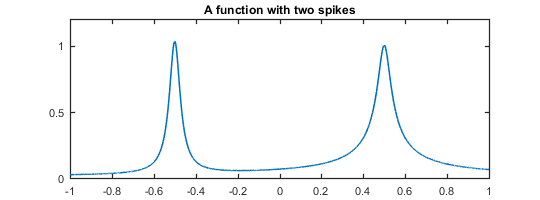
\includegraphics [width=4in]{chap3_04.png}
\begin{par}
 \vskip 1pt 
\end{par} \vspace{1em}
\begin{par}
Here are the Chebyshev coefficients of the chebfun.  This time, instead of \texttt{chebpoly} and \texttt{semilogy}, we execute the special command \texttt{chebpolyplot}, which has the same effect.
\end{par} \vspace{1em}
\begin{par}
 \vskip -2em 
\end{par} \vspace{1em}
\begin{verbatim}
chebpolyplot(f,'m'), grid on
title('Absolute values of Chebyshev coefficients',FS,9)
\end{verbatim}

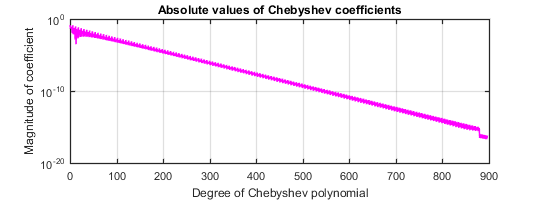
\includegraphics [width=4in]{chap3_05.png}
\begin{par}
 \vskip 1pt 
\end{par} \vspace{1em}
\begin{par}
Note that although it is far less wiggly, this function needs six times as many points to resolve as the previous one (Exercise 3.13). We shall explain these polynomial degrees in Chapter 8.
\end{par} \vspace{1em}
\begin{par}
Chebyshev interpolants are effective for complex functions (still defined on a real interval) as well as real ones.  Here, for example, is a complex function that happens to be periodic, though the Chebyshev representation does not take advantage of this fact.
\end{par} \vspace{1em}
\begin{par}
 \vskip -2em 
\end{par} \vspace{1em}
\begin{verbatim}
f = (3+sin(10*pi*x)+sin(61*exp(.8*sin(pi*x)+.7))).*exp(1i*pi*x);
\end{verbatim}
\begin{par}
A plot shows the image of $[-1,1]$ under $f$, which appears complicated:
\end{par} \vspace{1em}
\begin{par}
 \vskip -2em 
\end{par} \vspace{1em}
\begin{verbatim}
plot(f,'linewidth',0.6,'color',[0 .8 0]), axis equal off
\end{verbatim}

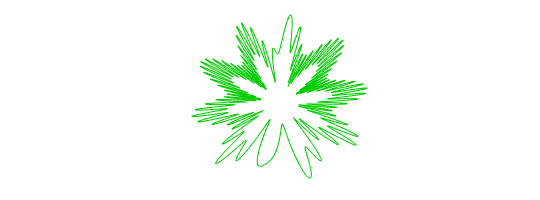
\includegraphics [width=4in]{chap3_06.png}
\begin{par}
 \vskip 1pt 
\end{par} \vspace{1em}
\begin{par}
Yet the degree of the polynomial is not so high:
\end{par} \vspace{1em}
\begin{par}
 \vskip -2em 
\end{par} \vspace{1em}
\begin{verbatim}
length(f)
\end{verbatim}

        \color{lightgray} \begin{verbatim}ans =
   614
\end{verbatim} \color{black}
    \begin{par}
People often ask, is there anything special about Chebyshev points and Chebyshev polynomials?  Could we equally well interpolate in other points and expand in other sets of polynomials?  From an approximation point of view, the answer is yes, and in particular, Legendre points and Legendre polynomials have much the same power for representing a general function $f$, as we shall see in Chapters 17--19.  Legendre points and polynomials are neither much better than Chebyshev for approximating functions, nor much worse; they are essentially the same. One can improve upon both Legendre and Chebyshev, shrinking the number of sample points needed to represent a given function by a factor of up to $\pi/2$, but to do so one must leave the class of polynomials.  See Chapter 22.
\end{par} \vspace{1em}
\begin{par}
Nevertheless, there is a big advantage of Chebyshev over Legendre points, and this is that one can use the FFT to go from point values to coefficients and back again.  There are algorithms that make such computations practicable for Legendre interpolants too [Piessens 1974, Alpert \& Rokhlin 1991, Dutt, Gu \& Rokhlin 1996, Potts, Steidl \& Tasche 1998, Iserles 2011]---see also Theorem 19.6 of this book---but Chebyshev remains the easy case.
\end{par} \vspace{1em}
\begin{par}

\begin{displaymath}
\framebox[4.7in][c]{\parbox{4.5in}{\vspace{2pt}\sl
{\sc Summary of Chapter 3.}
The Chebyshev polynomial $T_k(x)$ is an analogue for
$[-1,1]$ of the monomial $z^k$ on the unit circle.
Each Lipschitz continuous function $f$ on $[-1,1]$ has
an absolutely and uniformly convergent
Chebyshev series, that is, an expansion
$f(x) = a_0T_0(x) + a_1T_1(x) + \dots .$\vspace{2pt}}}
\end{displaymath}

\end{par} \vspace{1em}
\begin{par}
 \smallskip\small\parskip=2pt
{\bf Exercise 3.1.  Monomial and Chebyshev coefficients.} Let $p\in {\cal
P}_n$ have coefficient vectors $a = (a_0, a_1,\dots , a_n)^T$ for a
Chebyshev series and $b = (b_0, b_1,\dots , b_n)^T$ for a series in the
monomials $1, x, \dots , x^n$.  Show that $a$ and $b$ are related by $Aa
= b$, where $A$ is an upper-triangular matrix, whose entries you should
describe precisely, though you don't have to give
explicit formulas for them.
Prove that any $p\in {\cal P}_n$ has uniquely defined
coefficient vectors $a$ and $b$ for both representations.
\par
{\bf Exercise 3.2.  A Chebyshev coefficient.}  Use Chebfun to determine
numerically the coefficient of $T_5$ in the Chebyshev expansion of
$\tan^{-1}(x)$ on $[-1,1]$.
\par
{\bf Exercise 3.3.  Chebyshev coefficients and ``rat''.} (a) Use Chebfun
to determine numerically the coefficients of the Chebyshev series for $1
+ x^3 + x^4$.  By inspection, identify these rational numbers.  Use the
Matlab command {\tt [n,d] = rat(c)} to confirm this.  (b) Use Chebfun and
{\tt rat} to make good guesses as to the Chebyshev coefficients of $x^7/7
+ x^9/9$.  (Of course it is not hard to figure them out analytically.)
\par
{\bf Exercise 3.4.  Dependence on wave number.}
(a) Calculate the length
$L(k)$ of the chebfun corresponding to
$f(x) = \sin(kx)$ on $[-1,1]$ for $k = 1,2,4,8,\dots,2^{10}$.
(You can do this elegantly by defining a Matlab
anonymous function {\tt f = @(k)}....)
Make a loglog plot of $L(k)$ as a function of $k$ and comment
on the result.
(b) Do the same for $g(x) = 1/(1+(kx)^2)$.
\par
{\bf Exercise 3.5. Chebyshev series of a complicated function.}
(a) Make chebfuns of the three functions
$f(x) = \tanh(x)$,
$g(x) = 10^{-5}\tanh(10x)$,
$h(x) = 10^{-10}\tanh(100x)$ on $[-1,1]$, and call {\tt chebpolyplot}
to show their Chebyshev coefficients.  Comment on the results.
(b) Now define $s = f+g+h$ and comment on the result of
{\tt chebpolyplot} applied to $s$.  Chebfun does not automatically
chop the tail of a Chebyshev series obtained by summation, but applying the {\tt simplify}
command will do this.  What happens with
{\tt chebpolyplot(simplify(s))}?
\par
{\bf Exercise 3.6.  Chebyshev series of \boldmath $\hbox{\bf sign}(x)$ and $|x|$} [Bernstein 1914].
Derive the following Chebyshev series coefficients by using the first equality in (3.14).
(a) For $f(x) = \hbox{sign}(x)$, $a_k = 0$ for $k$ even and
$a_k = (4/\pi)(-1)^{k-1}/k$ for $k$ odd.
(b) For $f(x) = |x|$, $a_k = 0$ for $k$ odd, $a_0 = 2/\pi$, and
$a_k = (4/\pi)(-1)^{(k/2)}/(1-k^2)$ for $k\ge 2$ even.
\par
{\bf Exercise 3.7. Orthogonality of Chebyshev polynomials.} Equation
(3.12) gives the Chebyshev coefficient $a_k$ of $f$ by integration of $f$
against just the single Chebyshev polynomial $T_k$. This formula implies
an orthogonality property for $\{T_j\}$ involving a weighted integral.
State exactly what this orthogonality property is and show carefully how
it follows from the equations of this chapter.
\par
{\bf Exercise 3.8.  Conditioning of the Chebyshev basis.} Although the
Chebyshev polynomials are not orthogonal with respect to the standard
unweighted inner product, they are close enough to orthogonal
to provide a well-behaved
basis.  Set {\tt T = chebpoly(0:10)} and explore the Chebfun
``quasimatrix'' that results with commands like {\tt size(T)}, {\tt
spy(T)}, {\tt plot(T)}, {\tt svd(T)}. Explain the meaning of {\tt T} (you
may find Chapter 6 of the Chebfun Guide helpful) and determine the
condition number of this basis with {\tt cond(T)}.  (b) Now construct the
corresponding quasimatrix of monomials by executing {\tt x =
chebfun('x')}; {\tt M = T}; \verb|for j = 0:10, M(:,j+1) = x.^j; end|.
What is the condition number of {\tt M}?  (c) Produce a plot of these two
condition numbers for quasimatrices whose columns span ${\cal P}_n$
over $[-1,1]$ for $n =
0,1,\dots, 10$. (d) What happens to the condition numbers if $M$ is
constructed from monomials on $[0,1]$ rather than $[-1,1]$ via {\tt x =
chebfun('x',[0,1])}?
\par
{\bf Exercise 3.9.  Derivatives at endpoints.} Prove from (3.10) that the
derivatives of the Chebyshev polynomials satisfy $T_n'(1) = n^2$ for each
$n\ge 0$.  ({\em Markov's inequality} asserts that for any $p\in {\cal
P}_n$, $\|p'\| \le n^2 \|p\|$, where $\|\cdot\|$ is the supremum norm.)
\par
{\bf Exercise 3.10.  Odd and even functions.} Show that if $f$ is an odd
function on $[-1,1]$, its Chebyshev coefficients of even order are zero;
show similarly that if $f$ is even, its odd order coefficients are zero.
\par
{\bf Exercise 3.11.  A function neither even nor odd.} Apply
\verb|chebpolyplot| to the chebfun for $f(x) = \exp(x)/(1+10000x^2)$.  Why
does the plot have the appearance of a stripe?
\par
{\bf Exercise 3.12.  Extrema and roots of Chebyshev polynomials.}
Give formulas for the extrema and roots of $T_n$ in $[-1,1]$.
\par
{\bf Exercise 3.13.  Chebyshev coefficients and machine precision.} By a
command like \verb|f = chebfun('exp(x)',np)|, one can force Chebfun to
produce a chebfun of length \verb|np| (i.e., degree $\verb|np|-1$) rather
than determine the length automatically.  (a) Do this for the ``function
with wiggles'' of this section with $\verb|np|=257$, and comment on how
the {\tt chebpolyplot}
result differs from that shown in the text. (b) Likewise for the
``function with two spikes'' with $\verb|np|=2049$.
\par
{\bf Exercise 3.14.  Chebyshev series for a simple pole.}
(a) Let $t$ be a complex number with $|t|<1$ and define
$F(z) = (z-t)^{-1} + (z^{-1}-t)^{-1}$.  What is the Laurent series for $F\kern .5pt$?
(b) For the same $t$, show further that
$$ 1+2\sum_{k=1}^\infty t^k \kern .7pt T_k(x) = {1-t^2\over
1-2\kern .5pt tx+t^2}. \eqno (3.15) $$
(This formula can be interpreted as a generating function for
the Chebyshev polynomials.)
(c) Let $a\not\in [-1,1]$ be a real or complex number and let $t$ be
a real or complex number with $|t|<1$ such that $(t+t^{-1})/2 = a$.
Show that
$$ {1\over x-a} = {2\over t-t^{-1}}\left[
1+2\sum_{k=1}^\infty t^k \kern .7pt T_k(x)\right]. \eqno (3.16) $$
{\bf Exercise 3.15.  Chebyshev series of \boldmath$e^{ax}$.}
It can be shown that the Chebyshev series of $e^{ax}$ is
$$ e^{ax} = 2\sum_{k=0}^\infty {}' I_k(a) T_k(x) , \eqno (3.17) $$
where $I_k$ is the modified Bessel function of the first kind and
the prime indicates that the term $k=0$ is to be multiplied by $1/2$.
Derive the Chebyshev series for $\sinh(ax)$ and $\cosh(ax)$.
\par 
\end{par} \vspace{1em}



\end{document}
    
